\section*{Introduction}
Dans ce chapitre, nous présenterons le jeu de données et les analyses audio-MIDI. Nous ferons ensuite l’expérimentation théorique d’un \textit{système} implémentable qui devra être utilisé comme base de connaissances pour augmenter la rapidité et la qualité en sortie de Qparse. Enfin, nous présenterons les différentes contributions de développement.
\section{Le jeu de données}
Nous avons utilisé le Groove MIDI Dataset\footnote{\url{https://magenta.tensorflow.org/datasets/groove}} \cite{groove2019} (GMD) qui est un jeu de données mis à disposition par Google sous la licence Creative Commons Attribution 4.0 International (CC BY 4.0).\\
Le GMD est composé de 13,6 heures de batterie sous forme de fichiers MIDI et audio alignés. Il contient 1150 fichiers MIDI et plus de 22 000 mesures de batterie dans les styles les plus courants et avec différentes qualités de jeu. Tout le contenu a été joué par des humains sur la batterie électronique Roland TD-11 (figure \ref{electro_drums}).\newpage
\begin{figure}[h]
	\centering
	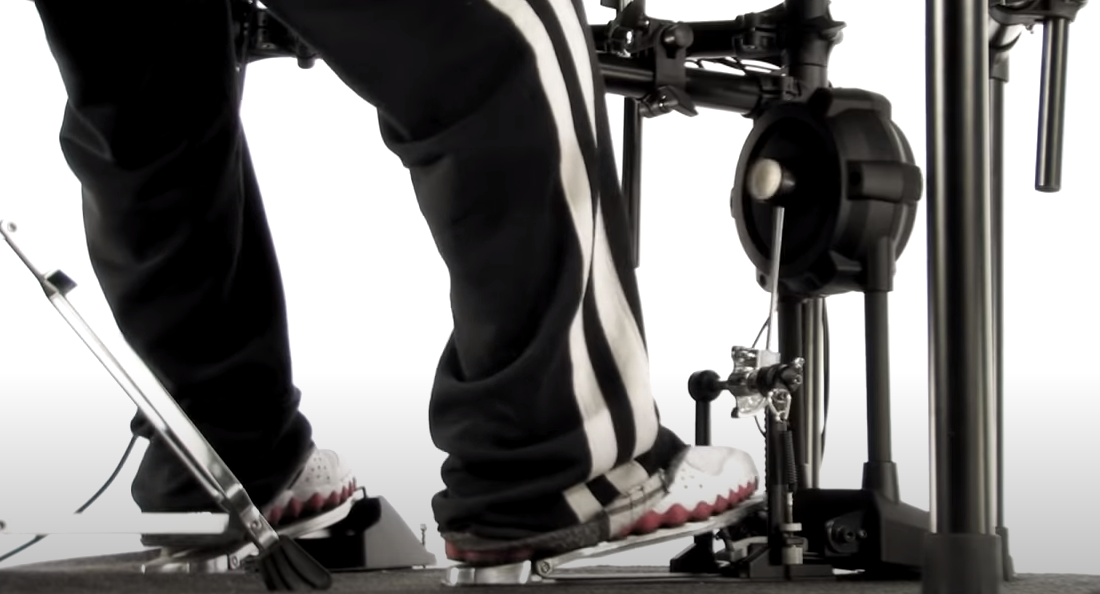
\includegraphics[height=35mm, width=60mm]{z_images/4_experimentations/0_groove/0_roland.png}\ \ 
	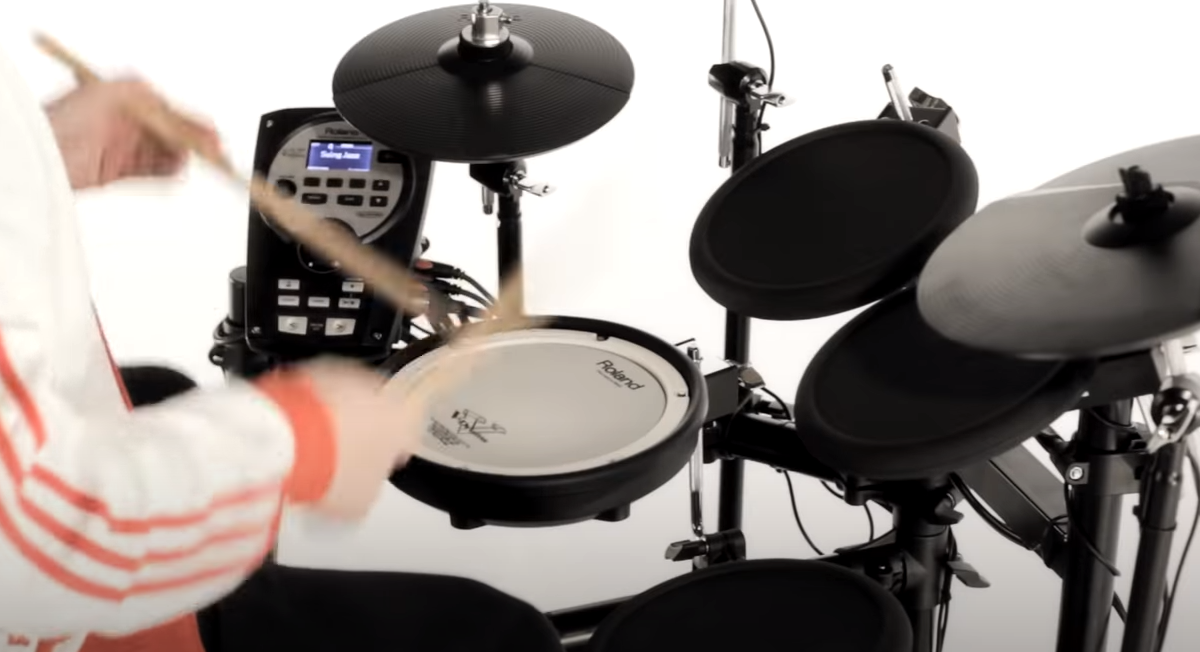
\includegraphics[height=35mm, width=60mm]{z_images/4_experimentations/0_groove/1_roland.png}
	\caption{Batterie électronique}
	\label{electro_drums}
	\textit{Source :} \url{https://www.youtube.com/watch?v=BX1V_IE0g2c}
\end{figure}
Autres critères spécifiques au GMD :
\begin{itemize}
	\item Toutes les performances ont été jouées au métronome et à un tempo choisi par le batteur.
	\item 80\% de la durée du GMD a été joué par des batteurs professionnels qui ont pu improviser dans un large éventail de styles. Les données sont donc diversifiées en termes de styles et de qualités de jeu (professionnel ou amateur).
	\item Les batteurs avaient pour instruction de jouer des séquences de plusieurs minutes ainsi que des fills\footnote{Un \textit{fill} est une séquence de relance dont la durée dépasse rarement 2 mesures. Il est souvent joué à la fin d’un cycle pour annoncer le suivant.}
	\item Chaque performance est annotée d’un style (fourni par le batteur), d’une métrique et d’un tempo ainsi que d’une identification anonyme du batteur.
	\item Il a été demandé à 4 batteurs d’enregistrer le même groupe de 10 rythmes dans leurs styles respectifs. Ils sont dans les dossiers eval-session du GMD.
	\item Les sorties audio synthétisées ont été alignées à 2 ms près sur leur fichier MIDI.
\end{itemize}
\subsection*{Format des données}
Le Roland TD-11 divise les données enregistrées en plusieurs pistes distinctes :
\begin{itemize}
	\item une pour le tempo et l’indication de mesure ;
	\item une pour les changements de contrôle (position de la pédale de charley) ;
	\item une pour les notes.\\
\end{itemize}
Les changements de contrôle sont placés sur le canal 0 et les notes sur le canal 9 (qui est le canal canonique pour la batterie).\\
Pour simplifier le traitement de ces données, ces trois pistes ont été fusionnées en une seule piste qui a été mise sur le canal 9.\\\\
« Control Changes
The TD-11 also records control changes specifying the position of the hi-hat pedal on each hit. We have preserved this information under control 4. »\\(\url{https://magenta.tensorflow.org/datasets/groove})\\$\Rightarrow$ ??? Je ne comprends pas encore comment trouver ce type d’informations dans les fichiers MIDI.\\L’utilisation de pretty\_midi devient urgente !
\section{Analyse MIDI-Audio}
\label{analyse_midi_audio}
Ces analyses ont été faites dans le cadre de transcriptions manuelles à partir de fichiers MIDI et Audio du GMD.
\subsection*{Comparaisons de transcriptions}
Pour les comparaisons de transcriptions, les transcriptions manuelles (TM) ont été éditées à l’aide de Lilypond\footnote{\url{http://lilypond.org/}} ou MuseScore\footnote{\url{https://musescore.com/}} et les transcriptions automatiques (TA) ont toutes été générées manuellement avec MuseScore.
\subsubsection{Exemple d’analyse 1}
\begin{figure}[h]
	\centering
	Transcription manuelle $\Rightarrow$ Transcription automatique
	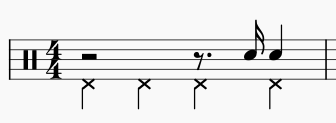
\includegraphics[height=20mm, width=50mm]{z_images/4_experimentations/1_analyse_midi_audio/0_drummer1_session3/1_manuelle.png}\ \ \ \ 
	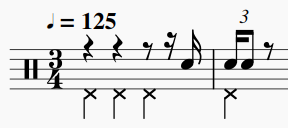
\includegraphics[height=20mm, width=45mm]{z_images/4_experimentations/1_analyse_midi_audio/0_drummer1_session3/0_musescore.png}
\end{figure}
\begin{itemize}
	\item Erreur d’indication de mesure (3/4 au lieu de 4/4) ;
	\item Les silences de la mesure 1 de la TA sont inutilement surchargés ;
	\item La noire du temps 4 de la mesure 1 de la TM est devenue les deux premières notes (une double-croche et une croche) d’un triolet sur le temps 1 de la mesure 2 de la TA.
\end{itemize}\newpage
\subsubsection{Exemple d’analyse 2}
\begin{figure}[h]
	\centering
	\tab Transcription manuelle $\Rightarrow$ Transcription automatique\\
	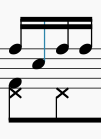
\includegraphics[height=20mm, width=13mm]{z_images/4_experimentations/1_analyse_midi_audio/0_drummer1_session3/5_manuelle.png}\ \ \ \ 
	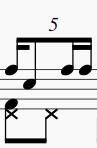
\includegraphics[height=20mm, width=13mm]{z_images/4_experimentations/1_analyse_midi_audio/0_drummer1_session3/4_musescore.png}
\end{figure}
\begin{itemize}
	\item Les doubles croches ont été interprétées en quintolet
	\item La deuxième double-croche est devenue une croche.\\
\end{itemize}
\subsubsection{Exemple d’analyse 3}
\begin{figure}[h]
	\centering
	Transcription manuelle $\Rightarrow$ Transcription automatique
	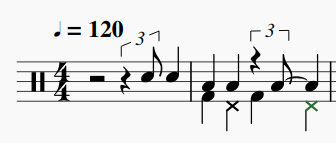
\includegraphics[height=24mm, width=50mm]{z_images/4_experimentations/1_analyse_midi_audio/0_drummer1_session3/3_manuelle.png}\ \ \ \ 
	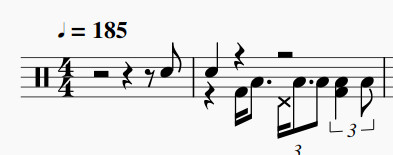
\includegraphics[height=25mm, width=55mm]{z_images/4_experimentations/1_analyse_midi_audio/0_drummer1_session3/2_musescore.png}
\end{figure}
\begin{itemize}
	\item Les grosses-caisses, les charleys et les caisses-claires ont été décalés d’un temps vers la droite.
	\item Les toms basses des temps 1 et 2 de la mesure 2 de la TM ont été décalés d’une double croche vers la droite dans la TA.
	\item La première caisse-claire de la mesure 1 devient binaire dans la TA alors qu’elle appartenait à un triolet dans la TM.
	\item Le triolet de tom-basse du temps 4 de la mesure 2 de la TA n’existe pas la TM.\\
\end{itemize}
\subsubsection{Exemple d’analyse 4}
\tab \tab Transcription manuelle $\Rightarrow$ Transcription automatique
\begin{figure}[h]
	\centering
	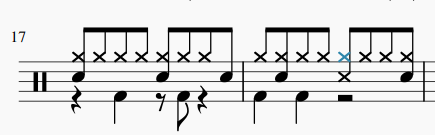
\includegraphics[height=19mm, width=50mm]{z_images/4_experimentations/1_analyse_midi_audio/1_drummer1_session1/3_manuelle.png}\ \ \ \ 
	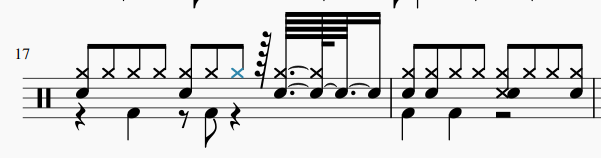
\includegraphics[height=19mm, width=70mm]{z_images/4_experimentations/1_analyse_midi_audio/1_drummer1_session1/2_musescore.png}
\end{figure}\\
Sur le temps 4 de la mesure 1, la deuxième croche a été transcrite d’une manière excessivement complexe !\newpage
\subsubsection{Exemple avec des flas}
Transcription manuelle\\
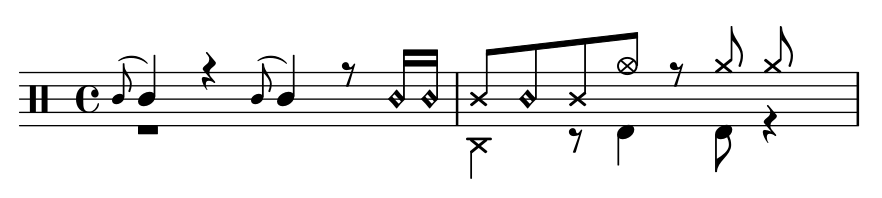
\includegraphics[height=25mm, width=95mm]{z_images/4_experimentations/1_analyse_midi_audio/2_transcriptions_flas/0_124_funk_95_fill_4-4.png}\\
Transcription automatique\\\\
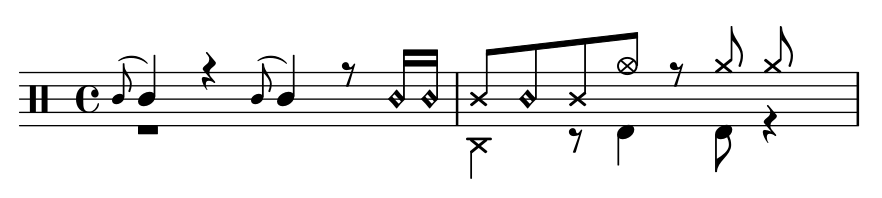
\includegraphics[height=20mm, width=130mm]{z_images/4_experimentations/1_analyse_midi_audio/2_transcriptions_flas/1_124_funk_95_fill_4-4.png}\\
\begin{itemize}
	\item Le premier fla est reconnu comme étant un triolet contenant une quadruple croche suivie d’une triple croche au lieu d’une seule note ornementée.
	\item Le deuxième fla est reconnu comme étant un accord.
	\item Les deux double en l’air sur le temps 4 de la TM sont mal quantifiée dans la TA. 
	\item La TA ne reconnaît qu’une mesure quand la TM en transcrit deux. En effet, la TA a divisé par deux la durée des notes afin de les faire tenir dans une mesure à 4 temps dont les unités de temps sont les noires. Par exemple, le soupir du temps 2 de la TM devient un demi-soupir sur le contre-temps du temps 1 dans la TA. Ou encore, la noire (pf, voir le tableau \ref{pitchs_instru}) sur le temps 1 de la mesure 2 de la TM suivie d’un demi-soupir devient une croche pointée sur le temps 3 de la TA.
	\item Autre problème : certaines têtes de notes sont mal attribuées. Par exemple, le charley ouvert en l’air sur le temps 2 de la mesure 2 de la TM devrait avoir le même symbole sur la TA. Idem pour les cross-sticks.
\end{itemize}\newpage
\subsection*{Transcription de partition}
\begin{figure}[h]
	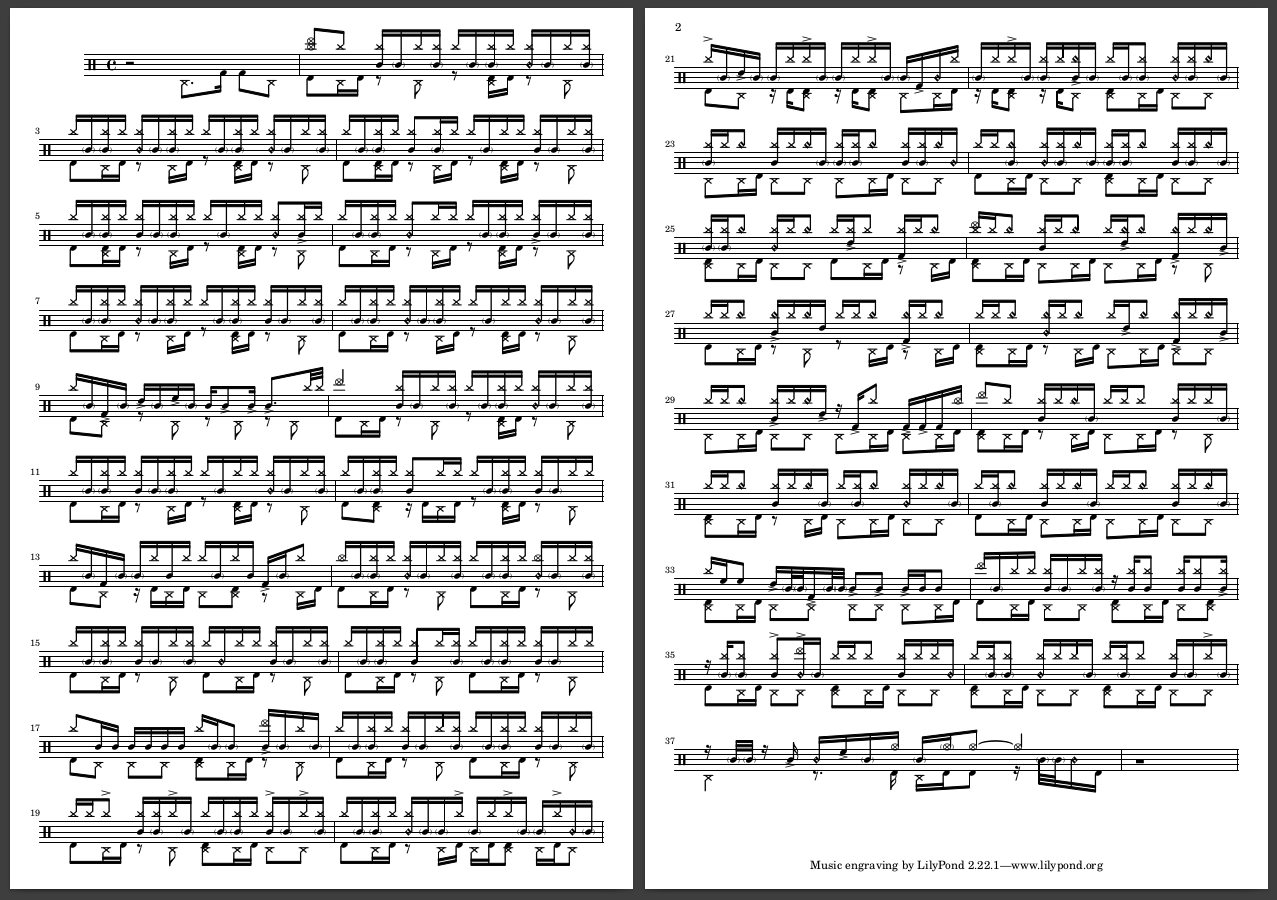
\includegraphics[height=120mm, width=160mm]{z_images/4_experimentations/1_analyse_midi_audio/3_partition.png}
	\caption{Partition de référence}
	\label{partition_ref}
\end{figure}
La figure \ref{partition_ref} est la transcription manuelle des fichiers \textit{004\_jazz-funk\_116\_beat\_4-4.mid} et \textit{004\_jazz-funk\_116\_beat\_4-4.wav} du GMD.\\Cette transcription a été entièrement faite avec Lilypond (voir le code lilypond sur le git \url{https://github.com/MartinDigard/Stage_M2_Inria})
Il s’agit d’une partition d’un 4/4 binaire dont le fichier MIDI est annoncé dans le GMD de style «jazz-funk» probablement en raison de la ride de type shabada rapide (le ternaire devient binaire avec la vitesse) combiné avec l’after-beat de type rock (caisse-claire sur les deux et quatre).\\
La transcription des données audio et MIDI contenues dans ces fichiers a permis une analyse plus approndie des critères à relever pour chaque évènement MIDI et de la manière de les considérer dans un objectif de transcription en partition lisible pour un musicien (Voir la section \ref{modelisation_transcription}).
\section{Expérimentation théorique d’un système}
Cette expérimentation théorique, basée sur la partition de référence de la figure \ref{partition_ref}, montre le procédé de création d’un \textit{système} et des règles qui en découlent (métrique, choix de grammaire, règles de séparation des voix et de simplification de l’écriture). Le \textit{système} devra ensuite être implémenté pour appliquer des tests qui seront effectués, dans un premier temps, sur la partition de référence.
\subsection*{Motifs et gammes}
\begin{figure}[h]
	\centering
	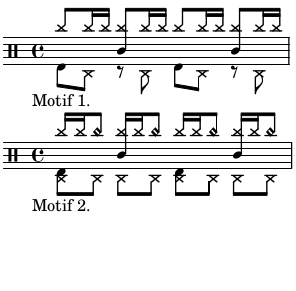
\includegraphics[height=43mm, width=40mm]{z_images/4_experimentations/2_experimentation_theorique/0_motifs_4-4_binaires.png}
	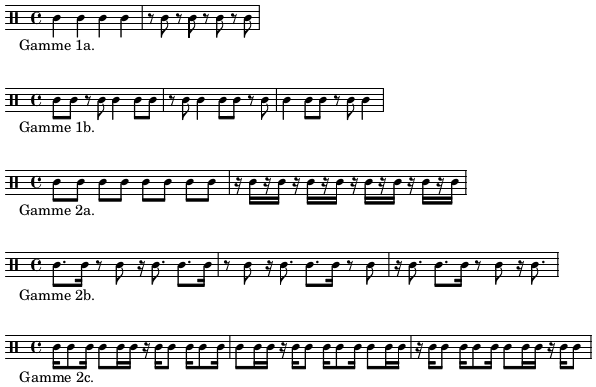
\includegraphics[height=55mm, width=85mm]{z_images/4_experimentations/2_experimentation_theorique/1_gammes_4-4_binaires.png}
	\caption{Motifs et gammes}
	\label{motifs_gammes}
\end{figure}
\subsubsection{Motifs}
À partir de la partition de référence, les deux motifs de la figure \ref{motifs_gammes} peuvent être systématisés. Le motif 1 est joué du début jusqu’à la mesure 18 avec des variations et des fills et le motif 2 est joué de la mesures 23 à la mesure 28 avec des variations. Ces deux motifs sont très classiques et pourront être détectés dans de nombreuses performances.\\
\subsubsection{Gammes}
Les gammes de la figure \ref{motifs_gammes} étayent toutes les combinaisons d’un motif en 4/4 binaires jusqu’aux doubles croches.\\
Les lignes 1 et 2 traitent les croches. La ligne 1 a 2 mesures dont la première ne contient que des noires et la deuxième que des croches en l’air. Ces deux possibilités sont combinées de manière circulaire dans les 3 mesures de la deuxième ligne.\\
Les lignes 3, 4 et 5 traitent les doubles-croches. La ligne 3 a 2 mesures dont la première ne contient que des croches et la deuxième que des doubles-croches en l’air. Ces deux possibilités sont combinées de manière circulaire dans les lignes 4 et 5 qui contiennent chacunes 3 mesures.
\subsection*{Systèmes — motifs et gammes combinés}
Pour la suite de l’expérimentation théorique, nous utiliserons le motif 1 de la figure \ref{motifs_gammes}.\\
\begin{figure}[h]
	\centering
	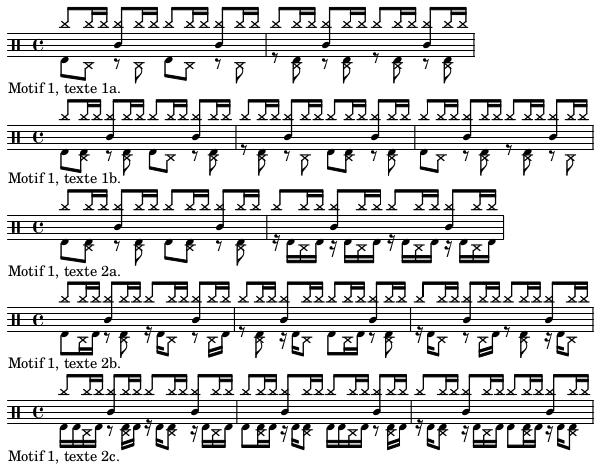
\includegraphics[height=75mm, width=85mm]{z_images/4_experimentations/2_experimentation_theorique/2_systeme_4-4_binaire.png}
	\caption{Partition d’un système en 4/4 binaire}
	\label{sys_binaire}
\end{figure}
\subsection*{Représentation du système en arbres de rythmes}
\label{demo_sys}
\begin{figure}[h]
	\centering
	\resizebox{350pt}{!} {
		\Tree[.Motif\ 1\ +\ gamme\ 1a
		[.Mesure\ 1
		[.Temps\ 1 [rd\\bd ][ [rd\\pf ][rd ]]]
		[.Temps\ 2 [rd\\cc ][ [rd\\pf ][rd ]]]
		[.Temps\ 3 [rd\\bd ][ [rd\\pf ][rd ]]]
		[.Temps\ 4 [rd\\cc ][ [rd\\pf ][rd ]]] ]
		[.Mesure\ 2
		[.Temps\ 1 [rd ][ [rd\\bd\\pf ][rd ]]]
		[.Temps\ 2 [rd\\cc ][ [rd\\bd\\pf ][rd ]]]
		[.Temps\ 3 [rd ][ [rd\\bd\\pf ][rd ]]]
		[.Temps\ 4 [rd\\cc ][ [rd\\bd\\pf ][rd ]]] ]]}
	\caption{Arbre de rythme — système}
	\label{arbre_sys}
\end{figure}
L’arbre de la figure \ref{arbre_sys} servira de base pour le suite de l’expérimentation. Comme indiqué à la racine de l’arbre, il représente la première ligne de la figure \ref{sys_binaire}. Même si cet arbre représente parfaitement le rythme concerné, il manque des indications de notation telles que les voix spécifiques à chaque partie du rythme ainsi que les choix d’écriture pour les distances qui séparent les notes de chaque voix entre elles en termes de durée.
\subsection*{Réécriture — séparation des voix et simplification}

\subsubsection{La séparation des voix}
Ainsi l’arbre syntaxique de départ est divisé en autant d’instruments qui le constituent et les voix seront regroupées en suivant les régles du système.
\begin{figure}[h]
	\centering
	\resizebox{350pt}{!} {
		\Tree[.Motif\ 1\ +\ Texte\ 1a
		[.Mesure\ 1
		[.Temps\ 1 [rd ][ [rd ][rd ]]]
		[.Temps\ 2 [rd\\cc ][ [rd ][rd ]]]
		[.Temps\ 3 [rd ][ [rd ][rd ]]]
		[.Temps\ 4 [rd\\cc ][ [rd ][rd ]]] ]
		[.Mesure\ 2
		[.Temps\ 1 [rd ][ [rd ][rd ]]]
		[.Temps\ 2 [rd\\cc ][ [rd ][rd ]]]
		[.Temps\ 3 [rd ][ [rd ][rd ]]]
		[.Temps\ 4 [rd\\cc ][ [rd ][rd ]]] ]]}
	\caption{Arbre de rythme — voix haute}
	\label{voix_haute}
\end{figure}\\
La voix haute regroupe la ride et la caisse-claire sur les ligatures du haut.
\begin{figure}[h]
	\centering
	\resizebox{350pt}{!} {
		\Tree[.Motif\ 1\ +\ Texte\ 1a
		[.Mesure\ 1
		[.Temps\ 1 [bd ][ [pf ][t ]]]
		[.Temps\ 2 [t ][ [pf ][t ]]]
		[.Temps\ 3 [bd ][ [pf ][t ]]]
		[.Temps\ 4 [t ][ [pf ][t ]]] ]
		[.Mesure\ 2
		[.Temps\ 1 [t ][ [bd\\pf ][t ]]]
		[.Temps\ 2 [t ][ [bd\\pf ][t ]]]
		[.Temps\ 3 [t ][ [bd\\pf ][t ]]]
		[.Temps\ 4 [t ][ [bd\\pf ][t ]]] ]]}
	\caption{Arbre de rythme — voix basse}
	\label{voix_basse}
\end{figure}\\
La voix basse regroupe la grosse-caisse et le charley au pied sur les ligatures du bas.
\subsubsection{Les règles de simplifications}
L’objectif des simplifications est de réécrire les écarts de durées qui séparent les notes d’une manière appropriée pour la batterie et qui soit la plus simple possible.\\
Pour la notation soit appropriée à la batterie, il faut que les ligatures relient les notes d’un temps entre elles (rendre la pulse visuelle).\\\\
Pour les figures ci-dessous :
\begin{itemize}
	\item x = une note ;
	\item r = un silence ;
	\item t = une continuation (point ou liaison)
\end{itemize}
Simplifier l’écriture de chaque voix (\textit{Règles établis par le système})
\begin{figure}[h]
	\centering
	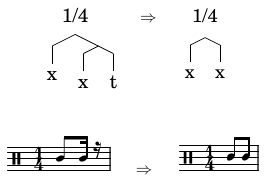
\includegraphics[height=40mm, width=55mm]{z_images/4_experimentations/2_experimentation_theorique/simpl.png}
\end{figure}\\
\begin{figure}[h]
	\centering
	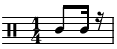
\includegraphics[height=10mm, width=25mm]{z_images/4_experimentations/2_experimentation_theorique/simplification_0.png}\ \ \ \ \ $\Rightarrow$\ \ \ \ \
	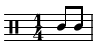
\includegraphics[height=10mm, width=20mm]{z_images/4_experimentations/2_experimentation_theorique/simplification_1.png}
\end{figure}
\begin{figure}[h]
	\centering
	\resizebox{50pt}{!} {
		\Tree[.1/4 [x ][ [x ][t ]] ]
	}\ \ \ \ \ $\Rightarrow$\ \ \ \ \
	\resizebox{30pt}{!} {
		\Tree[.1/4 [x ][x ] ]
	}
\end{figure}

\begin{figure}[h]
	\centering
	\resizebox{70pt}{!} {
		\Tree[.1/4 [t ][x ][x ][x ] ]
	}\ \ \ \ \ $\Rightarrow$\ \ \ \ \
	\resizebox{70pt}{!} {
		\Tree[.1/4 [r ][x ][x ][x ] ]
	}
\end{figure}
\begin{figure}[h]
	\centering
	\resizebox{70pt}{!} {
		\Tree[.1/4 [x ][t ][x ][x ]]
	}\ \ \ \ \ $\Rightarrow$\ \ \ \ \
	\resizebox{50pt}{!} {
		\Tree[.1/4 [x ][ [x ][x ]]]
	}
\end{figure}
\begin{figure}[h]
	\centering
	\resizebox{70pt}{!} {
		\Tree[.1/4 [t ][x ][x ][t ] ]
	}\ \ \ \ \ $\Rightarrow$\ \ \ \ \
	\resizebox{50pt}{!} {
		\Tree[.1/4 [ [r ][x ]][x ] ]
	}
\end{figure}
\begin{figure}[h]
	\centering
	\resizebox{50pt}{!} {
		\Tree[.1/4 [t ][ [x ][x ]]]
	}\ \ \ \ \ $\Rightarrow$\ \ \ \ \
	\resizebox{50pt}{!} {
		\Tree[.1/4 [r ][ [x ][x ]]]
	}
\end{figure}
\begin{figure}[h]
	\centering
	\resizebox{50pt}{!} {
		\Tree[.1/4 [t ][ [x ][t ]] ]
	}\ \ \ \ \ $\Rightarrow$\ \ \ \ \
	\resizebox{30pt}{!} {
		\Tree[.1/4 [r ][x ] ]
	}
\end{figure}
\newpage
\subsection*{Objectif de cette expérimentation théorique}
La méthode des \textit{systèmes} étant basée sur une approche dictionnaire, cette expérimentation théorique a pour but d’orienter la recherche d’autres systèmes par observation du jeu de données et de montrer comment les construire pour agrandir la base de connaissance de Qparse pour l’ADT.
\newpage
\section{Développement}
\subsection*{DrumCode}
Adaptation de la modélisation pour la transcription en cpp.
\subsection*{Tests unitaires sur les Jams}
\label{jam_tests}
Les Jams permettent de passer du monophonique au polyphonique.
\subsection*{Parsing}
\label{gram_pond}
Tests effectués avec le fichier midi suivant :\\\\
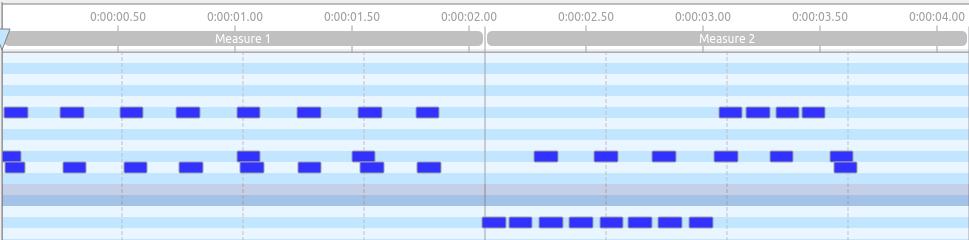
\includegraphics[height=50mm, width=160mm]{z_images/4_experimentations/3_developpement/0_midi_2bars_fill.png}\\\\
%\textit{Voix basse}\\
Un premier test convaincant est effectué avec la grammaire suivante :\\\\
// bar level\\
0 -> C0                1\\
0 -> E1                1\\
0 -> U4(1, 1, 1, 1)    1\\

// half bar level\\
9 -> C0                1\\
9 -> E1                1\\

// beat level\\
1 -> C0                1\\
1 -> E1                1\\
1 -> T2(2, 2)          1\\
1 -> T4(4, 4, 4, 4)    1\\

// croche level\\
2 -> C0                1\\
2 -> E1                1\\

// double level\\
4 -> C0                1\\
4 -> E1                1\\
4 -> E2                1\\
4 -> T2(6, 6)          1\\

// triple level\\
6 -> E1                1\\\\
Cette grammaire sépare les ligatures par temps au niveau de la mesure. Puis, au niveau du temps, elle autorise les divisions par deux (croches) et par quatre (doubles-croches). Tous les poids sont réglés sur 1. L’arbre de parsing en résultant est considéré comme « convaincant » car il découpe correctement les mesures et les temps.
\\\\
\resizebox{450pt}{!} {
\Tree[.Mesure\ 1
[.Temps\ 1 [0-ON\\1-ON\\2-ON ][3-OFF\\4-OFF\\5-OFF ][6-ON\\7-ON ][8-OFF\\9-OFF ]]
[.Temps\ 2 [10-ON\\11-ON ][12-OFF\\13-OFF ][14-ON\\15-ON ][16-OFF\\17-OFF ]]
[.Temps\ 3 [18-ON\\19-ON\\20-ON ][21-OFF\\22-OFF\\23-OFF ][24-ON\\25-ON ][26-OFF\\27-OFF ]]
[.Temps\ 4 [28-ON\\29-ON\\30-ON ][31-OFF\\32-OFF\\33-OFF ][34-ON\\35-ON ][36-OFF\\37-OFF ]]
]}\\\\\\
Les temps de la première mesure du fichier MIDI sont bien quantifié mais ceux de la deuxième mesure présentent quelques défauts de quantification visibles dès le premier temps.\\\\
\resizebox{300pt}{!} {
\Tree[.Mesure\ 2
[.Temps\ 1 [38-ON ][ [39-OFF ][40-ON ] ][ [41-OFF\\42-ON ][43-ON ] ][ [44-OFF\\45-OFF ][46-ON ] ]]
]}\\\\\\
Les Onsets sont correctement triés au niveau des doubles croches mais certaines doubles croches sont inutilement subdivisées en triples croches (les 2ème, 3ème et 4ème doubles croches sur le premier temps ci-dessus).\\\\
\textbf{2ème exemple :}\\
Après une augmentation du poids des triples croches dans la grammaire (monté de 1 à 5)et une baisse de tous les autres poids (descendu de 1 à 0.5), et mis à part le troisième temps de la 2ème mesure, tous les Onsets sont bien triés et aucuns ne sont subdivisés.






%\newpage
%\section{Résultats et discussion}
%\subsection{Résultats}
%\subsection{Évaluation}
%1 - Transcription manuelle à partir de fichier midi et/ou wav d’une partition contenant des systèmes. Écriture des systèmes contenues dans la partition (arbres, séparation des voix, réécriture)\\\\

\section*{Conclusion}
Conclusion de ce chapitre.